
Similarly to the PAMAM/PPI-Janus (see Section \ref{PAMAM/PPI-Janus}), this tutorial aims to build a dendrimer in which each side of the dendrimer is composed by BBs of a different dendrimer.
However, differently to the PAMAM/PPI-Janus tutorial, here the molecule is supposed to be completely divided between PAMAM and PPI side.
That is, even the core block is split (Figure \ref{fig:Half}).

\begin{figure}
    \centering
    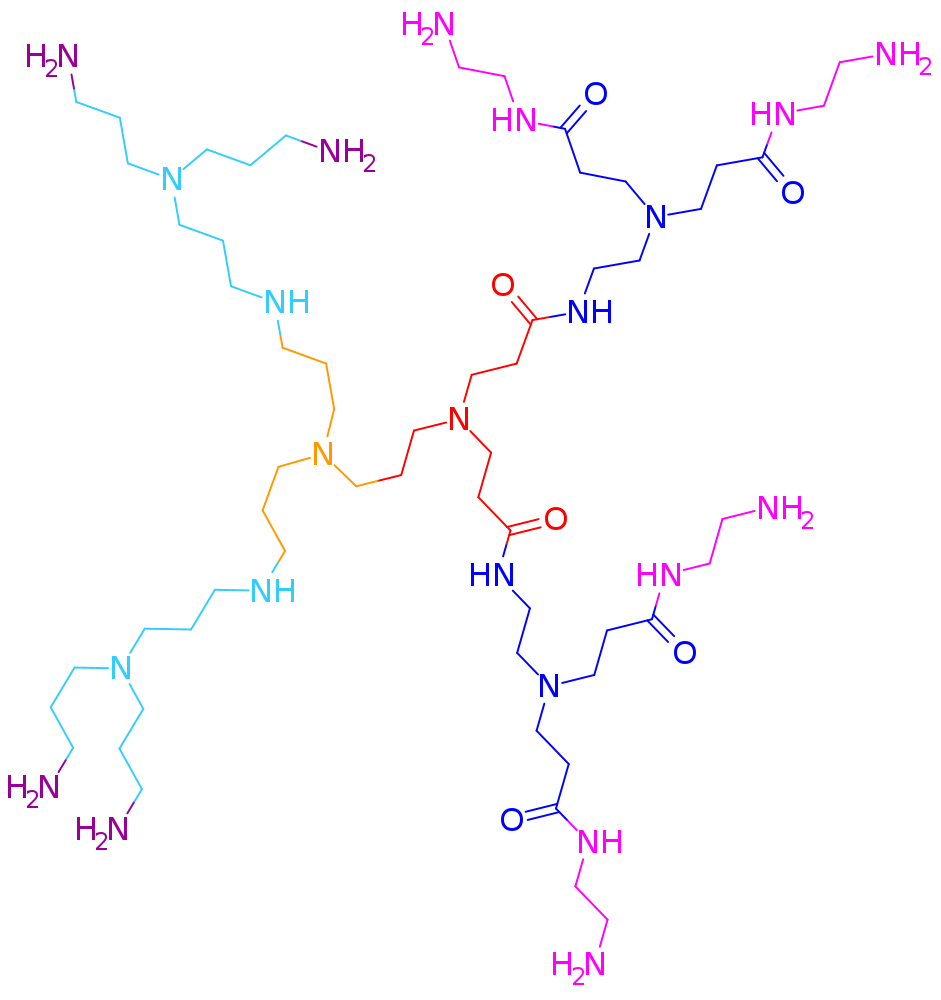
\includegraphics[width=0.4\textwidth]{PAMAM_PPI-half/PAMAMPPIPOL.png}
    \caption{PAMAM/PPI dendrimer in which each side is composed by either PAMAM or PPI dendrimer. The PAMAM core block is illustrated in red, intermediary and core blocks are displayed in blue and pink, respectively. PPI part is displayed in orange, cyan and purple for core, intermediary and terminal BBs, respectively. }
    \label{fig:Half}
\end{figure}

All needed files are provided in demo directory:

\begin{lstlisting}
<path/to/pypolybuilder>/demo/gromacs_format/polymer/PAMAM_PPI_Half
\end{lstlisting}
\dirtree{%
.1 PAMAM\_PPI\_Half.
.2 coreHalf\_PAMAM.itp.
.2 coreHalf\_PPI.itp.
.2 inter\_PAMAM.itp.
.2 inter\_PPI.itp.
.2 ter\_PAMAM.itp.
.2 ter\_PPI.itp.
.2 list\_param.itp.
.2 connect.in.
.2 run.
.3 PAMAM\_PPI\_Half.sh.
.3 PAMAMPPI.top.
.3 mdp.
}

All the following procedure for building the molecule with a side using only PAMAM BBs and the other side using only PPI BBs, is automated in a available bash file called \texttt{how\_to\_run\_this\_example.txt}.

In order to do that, we created separated topology files of the core block for each side of the dendrimer, \texttt{coreHalf\_PAMAM.itp} and \texttt{coreHalf\_PPI.itp}.
Intermediary and terminal blocks are the same as used in PAMAM and PPI tutorials (See Figure \ref{fig:HalfBBs}).

\begin{figure}
    \centering
    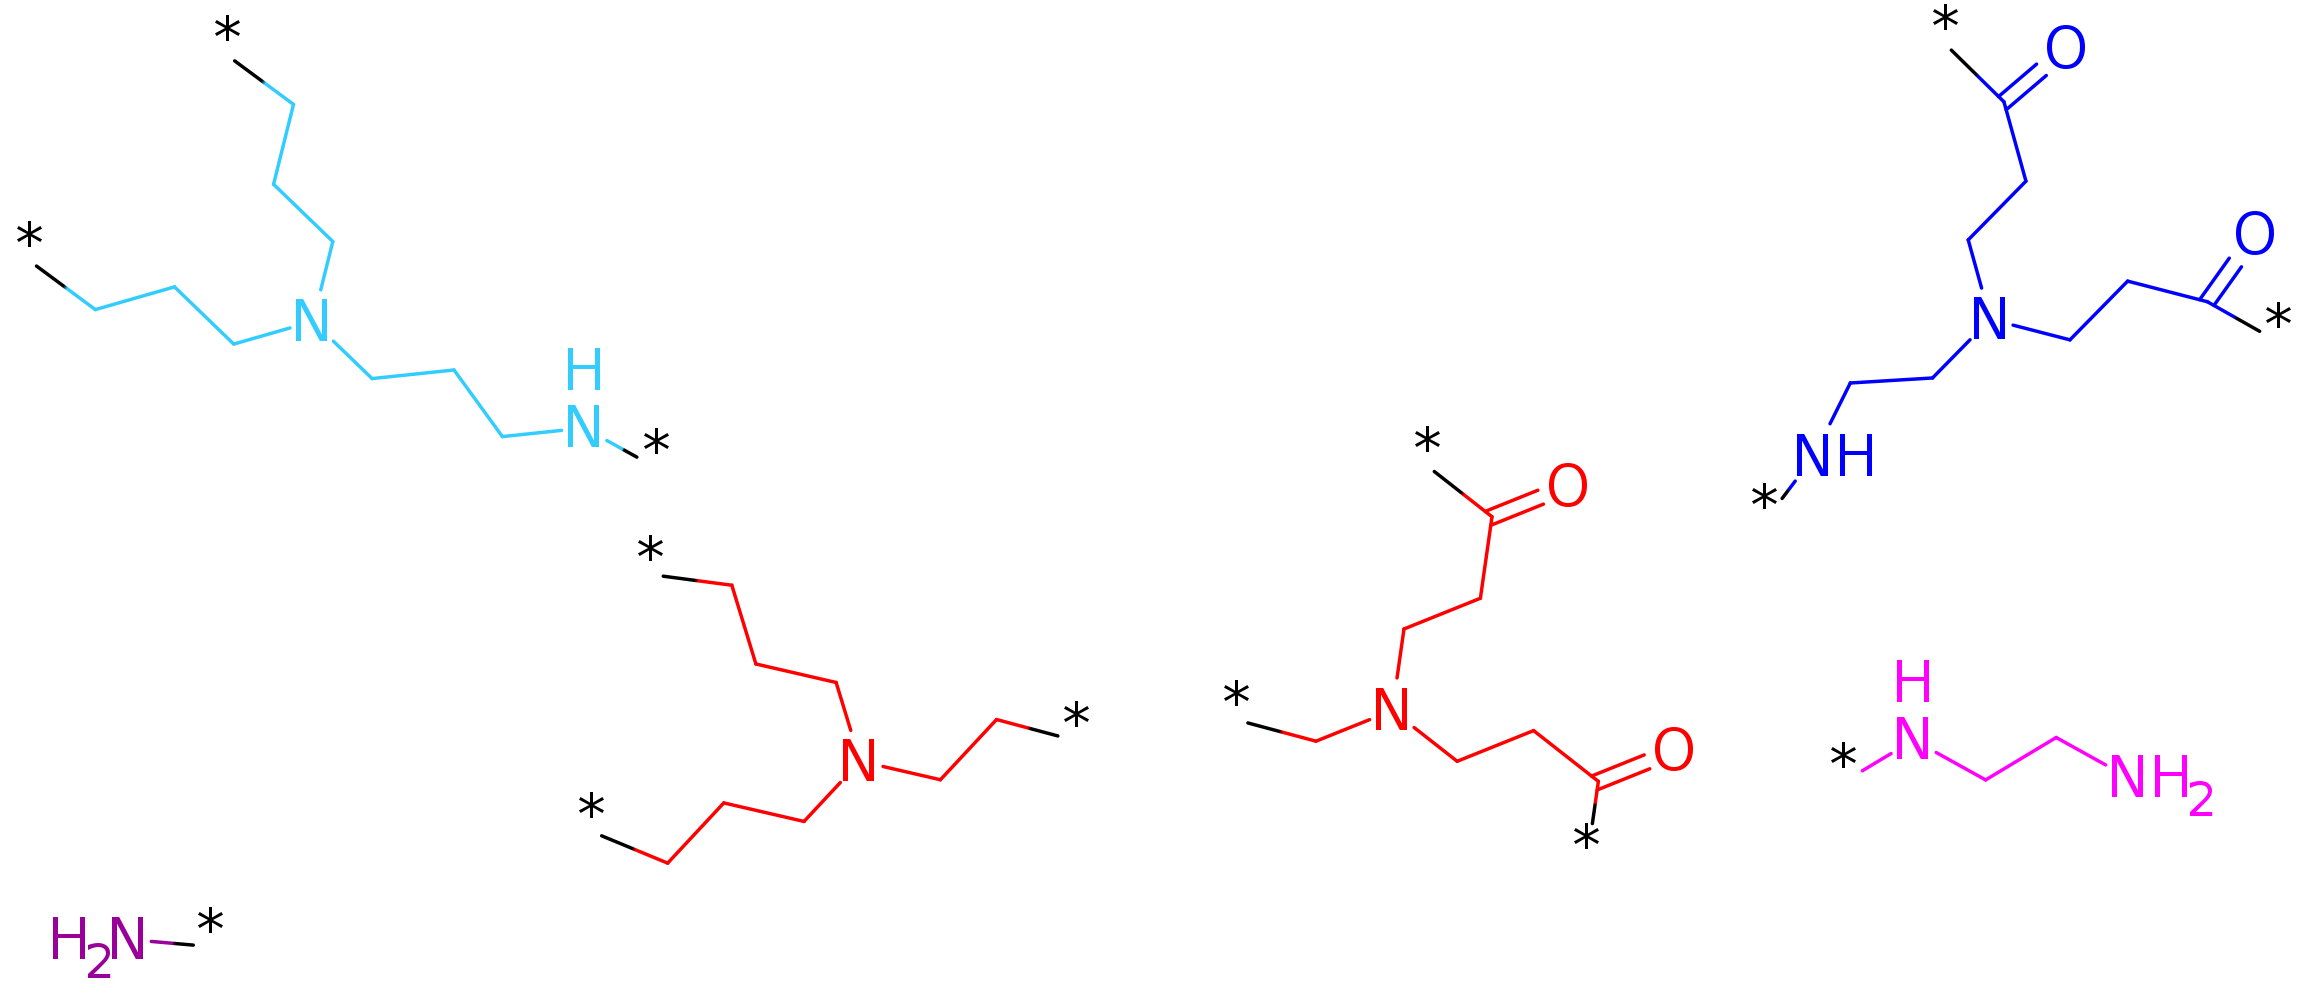
\includegraphics[width=\textwidth]{PAMAM_PPI-half/PAMAMPPIBBs.png}
    \caption{PAMAM/PPI dendrimer in which each side is composed of PAMAM or PPI. PAMAM BBs are illustrated on the right where the core block is illustrated in red, intermediary and core blocks are displayed in blue and pink, respectively. PPI part is on the left and displayed in orange, cyan and purple for core, intermediary and terminal BBs, respectively.}
    \label{fig:HalfBBs}
\end{figure}

Therefore, firstly each half will be built using the dendrimer module by using the following command lines:

\begin{lstlisting}
python3 ../../../../__main__.py \
--core=coreHalf_PAMAM.itp \
--inter=inter_PAMAM.itp \
--ter=ter_PAMAM.itp \
--params=list_param.itp \
--ngen=1 \
--name=PAMH \
--output=PAMAMhalf.itp \
--nogeom \
--dendrimer
\end{lstlisting}

To build the first side using PAMAM BBs.
Here the usage of dendrimer module is exactly the same as when generating a whole dendrimer.
The only difference is that at the core BB, the \texttt{[ branches ]} field tells pyPolyBuilder that only the two available branching points will be used.

\begin{lstlisting}
[ branches ]
;  donor   acceptor
    0      6
    0      9
\end{lstlisting}

Secondly, PPI half is built.
The procedure is similar to the one for building the PAMAM half:

\begin{lstlisting}
python3 ../../../../__main__.py \
--core=coreHalf_PPI.itp \
--inter=inter_PPI.itp \
--ter=ter_PPI.itp \
--params=list_param.itp \
--ngen=1 \
--name=PPIH \
--output=PPIhalf.itp \
--nogeom
\end{lstlisting}

In both calls of pyPolyBuilder, the option \texttt{--nogeom} was used since we're not interested in optimizing the geometry for an intermediary molecule. 
Hence, this options can be used to save time skipping the optimization step and the generation of a coordination file for the intermediary molecules.

\begin{figure}
    \centering
    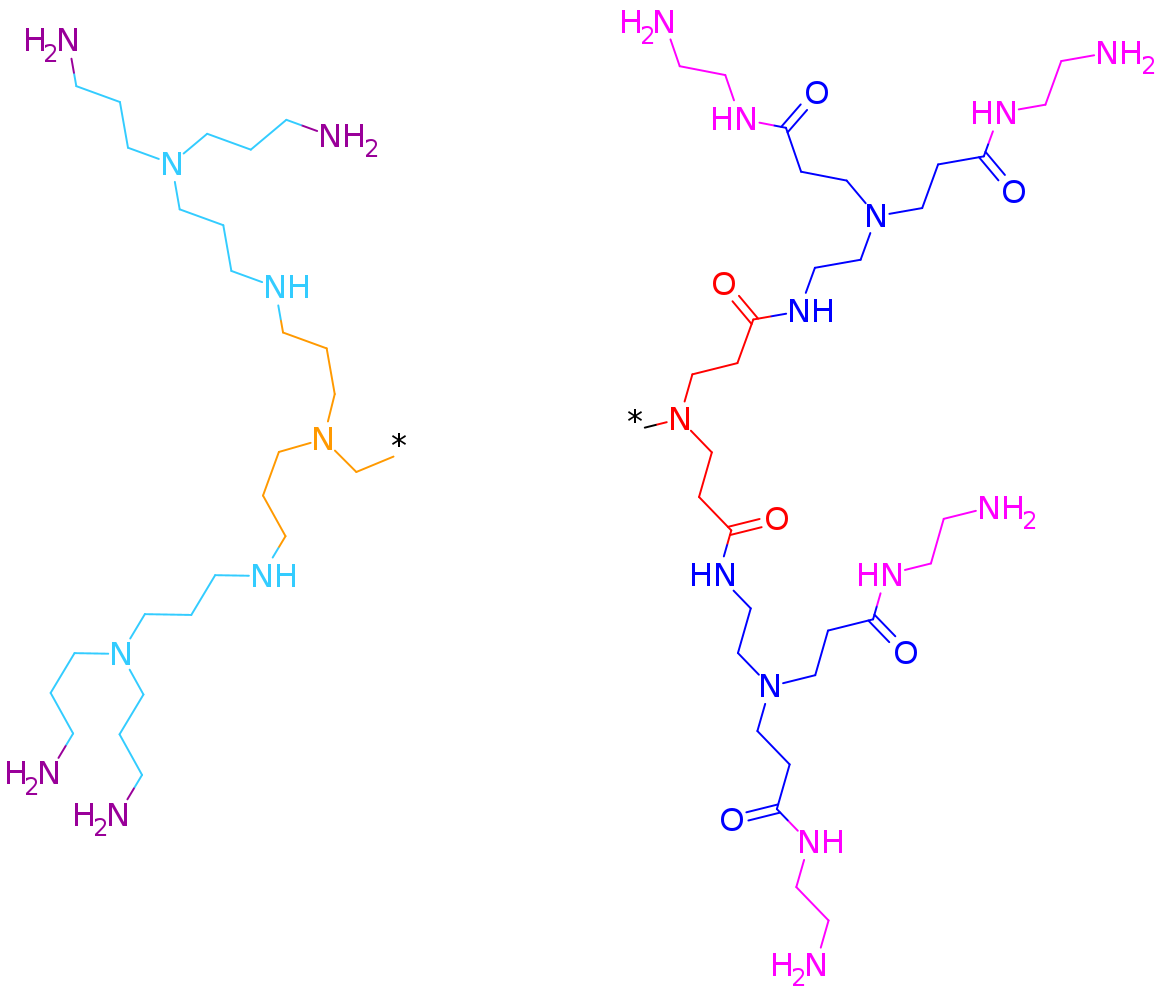
\includegraphics[width=0.5\textwidth]{PAMAM_PPI-half/PAMAMPPIHalfs.png}
    \caption{PAMAM/PPI dendrimer in which each side is composed by either PAMAM or PPI dendrimer. The PAMAM core block is illustrated in red, intermediary and core blocks are displayed in blue and pink, respectively. PPI part is displayed in orange, cyan and purple for core, intermediary and terminal BBs, respectively. }
    \label{fig:HalfHalf}
\end{figure}

Once both halfs are done, one will have the MTFs for each side of the dendrimer (see Figure \ref{fig:HalfHalf}.
Now these two parts need to be connected by using the network module.
In order to do that, the \texttt{connect.in} file simply uses both sides and connect the fist atom of each topology.

\begin{lstlisting}
#[ BUILDING BLOCKS ]
1       PAMH
2       PPIH

#[ CONNECTS ]
1       2       1       1
\end{lstlisting}

Connecting both sides, the final molecule will be generated (Figure \ref{fig:HalfHalf}).
The command line to connect the dendrimer is the following one:

\begin{lstlisting}
python3 ../../../../__main__.py \
--bbs=PAMAMhalf.itp,PPIhalf.itp \
--in=connect.in \
--params=list_param.itp \
--name=PAMPPI \
--output=PAMAMPPI.itp \
--gro=PAMAMPPI.gro \
--nsteps 500 \
--network
\end{lstlisting}

Once this last command line is executed, the dendrimer will be readily prepared, including its geometry optimized in vacuum (Figure \ref{fig:HalfPPB}).
In this tutorial, the internal pseudo-force field of pyPolyBuilder was used, so it is strongly suggested that after building any molecule in pyPolyBuilder, a MD simulation package should be used to minimize the energy using an actual force field (if the option \texttt{--forcefield} was not used in pyPolyBuilder) and to equilibrate the molecule in the desired solvent.

\begin{figure}
    \centering
    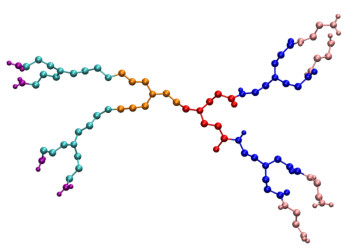
\includegraphics[width=0.5\textwidth]{PAMAM_PPI-half/PAMAMPPIPPB.pdf}
    \caption{PAMAM/PPI dendrimer in which each side is composed by either PAMAM or PPI dendrimer. The PAMAM core block is illustrated in red, intermediary and core blocks are displayed in blue and pink, respectively. PPI part is displayed in orange, cyan and purple for core, intermediary and terminal BBs, respectively. }
    \label{fig:HalfPPB}
\end{figure}

To mimic the procedure of energy minimization, equilibration and simulation, the run directory was provided where the script \texttt{PAMAM\_PPI\_half.sh} can be used to automate the whole process.
The outputs from pyPolyBuilder \texttt{PAMAMPPI.*} need to be copied to the run directory and the \texttt{PAMAM\_PPI\_half.sh} need to be changed to include an actual path for a gromacs package.
By running \texttt{PAMAM\_PPI\_half.sh}, it will automatically solvate the molecule, minimize the energy of the system, equilibrate it for 100 ps in nvt and npt ensembles and carry out 100 ps of molecular dynamics simulation.
An equilibrated structure is shown in Figure \ref{fig:HalfSOL}.

\begin{figure}
    \centering
    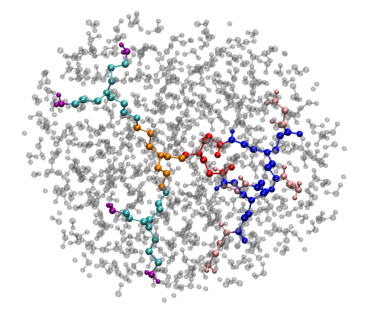
\includegraphics[width=0.5\textwidth]{PAMAM_PPI-half/PAMAMPPISOL.pdf}
    \caption{PAMAM/PPI dendrimer in which each side is composed of either PAMAM or PPI in water. The color scheme for the dendrimer is in accordance with Figure \ref{fig:HalfPPB} and water molecules are translucent in silver.}
    \label{fig:HalfSOL}
\end{figure}